\documentclass[../dejiny-rodu-prusiku.tex]{subfiles}

\begin{document}

% str 55 @ 69
\section{Odnož Horní Bříza I I I - větve Výrov}

Potomci Tomáše Prusíka, rodáka z Výrova.

1812 - 1897

Čtvrtým dítětem rychtáře Vojtěcha Prusíka a jeho ženy Anny byl syn Tomáš, narodil se 19. 11. 1812. Bylo to v době po porážce Napoleonově u Lipska. Když bylo v pozdějších letech určeno, že rodný grunt ve Výrově dosta­ne nejmladší syn Václav, začala se hledat nevěsta pro dospívajícího Tomáše. Tomášovi se nechtělo dlouho do ženitby a doma byl nejvýše spokojen. Protože však bylo dětí mnoho, neušel odchodu z domova. Dvě jeho sestry Anna a Rosalie byly již provdané v Horní Bříze a tam také našly nevěstu svému bratrovi. Byla to Kateřina Beránková z gruntu č. 26. Narodila se v roce 1816 na statku, jemuž se říkalo postaru "Fakanovský". První zápis v gruntovní knize o této usedlosti je ze 14. 3. 1662, kdy byl majitelem kovář Kabát. V roce 1790 byl již majitelem Antonín Beránek. Sem se 24. 2. 1835 přiženil z Výrova Tomáš Prusík. Družka jeho života, Kateřina Beránková předešla ho ve smrti o 18 let, zemřela 20. 5. 1879 v Horní Bříze. Výměnkář Tomáš Prusík zemřel tam ve stáří 87 let dne 19. dubna 1897.

Tomáš byl velmi uvážlivý sedlák, spíše konservativního ražení a některým moderním směrům nebyl vždy rychle přístupný. Mnoho let se mu v Horní Bříze stýskalo po domově a často, nejen o poutích a jiných významných příležitostech, sebral se a putoval pěšky do Výrova. Zvláštní pozornost budíval tím, že místo řemenu míval kolem pasu povříslo. Tomáš s Kateřinou měli devět dětí, které dospěly.

Nejstarším dítětem byl syn Jan. Narodil se 17. 5. 1840 v Horní Bříze, byl profesorem filologie, působil mimo jiné v Rusku, kde se utopil v r. 1875. Druhá byla dcera Marie, provdaná Krausová v nedaleké obci Nevřeni č. 48. Narodila se 19. 3. 1844 v Horní Bříze a zemřela 23. 4. 1904 v Nevřeni. Třetím dítětem byla Anna narozená 22. 1. 1847. I ona byla provdaná Krausová v Nevře­ni č. 7, ale tam zemřela jako čtyřicetiletá 14. 3. 1887. Druhým synem byl Tomáš, nar. 5. 8. 1849 v Horní Bříze, stal se knězem a zemřel 16. 7. 1903 v Dolních Břežanech u Zbraslavě. Pak byla dcera Kateřina provdaná Schneibergová v Plzni. Narodila se 3. 8. 1856 v Horní Bříze a zemřela v Plzni 30. 6. 1942. Dožila se nejdelšího věku ze svých sourozenců. Čtvrtou dcerou Tomáše Prusíka byla Josefa. Narodila se 27. 7. 1857 v Horní Bříze, neprovdala se a zemřela za tuhé zimy 24. 1. 1929 ve svém rodišti. Syn Václav nar. 8. 3. 1858 zemřel jako svobodny 1. 6. 1840 v Horní Bříze. Jeho bratr Blažej nar. 7. 1. 1861 byl prvním držitelem gruntu po otci. Zemřel již ve věku 42 let dne 27. 3. 1903 v Horní Bříze. Druhým držitelem se stal po něm jeho bratr Josef nar. 11. 3. 1863. Zemřel za dva dny po svém bratru Václavovi 3. 6. 1940.

% str 56 @ 70
Nejstarší syn Tomáše Prusíka a jeho ženy Kateřiny jmenoval se Jan a narodil se 17. 5. 1840 v Horní Bříze č. 26. Jako první využil dobrodiní svého strýčka vikáře Blažeje Prusíka v Praze, Na Hradčanech a přišel studovat na staroměstské gymnasium do Prahy. Studoval pak klasickou filologii na universitě. Vedle češtiny a němčiny učil latině, řečtině i dějepisu. Jan Prusík se stal nejdříve suplentem na gymnasiu v Plzni, od roku 1873 učil v Sučavě, ležící v tehdejší Bukovině v Rakousko-Uhersku. Od roku 1865 do 1866 učil v České Lípě. Na podzim roku 1868, tedy před sto lety, stal se řádným profesorem právě založeného nižšího gymnasia v Třeboni. Profesor Jan Prusík byl menším rebelantem, nebyl spokojen s platem a své slavjanofilství dával příliš na odiv. To se ovšem nelíbilo c.k. ministerstvu osvěty a dalo Jana Prusíka, do tzv. příkaznosti. Dnes by se tomu řeklo, že byl dočasně zbaven místa. Stalo se t0 23. září 1870. Předtím se Jan Prusík oženil 29. 2. 1870 s Marií Magda­lenou Ottovou, dcerou mlynáře z Třemošné u Plzně. Man­želství toto nebylo však příliš šťastné. Jeho žena narodila se v r. 1843 ve mlýně v Třemošné č. 48, dala svému manželi jednoho synka, ale zemřela v Třemošné na souchotiny již 12. 4. 1873. V té době byl již Jan Prusík v Rusku. Tehdy tam odešlo mnoho Čechů jako řemeslníci, podnikatelé, hudebníci, učitelé a jiní. Byli tam velmi vítáni.

Jan Prusík učil v Rusku také filologii v některém městě na Volze. Bohužel, nepodařilo se zjistiti přesné místo jeho působiště. Pobyl tam asi čtyři roky a nikdy se již domů nevrátil. Jeho žena s ním do Ruska jeti nechtěla a zůstala s děckem u rodičů. Podle starých pamětníků utopil se Jan Prusík ve Volze v r. 1875. Dostal křeč při koupání. Stalo se to v Kazani. V popisu jeho osoby, což je zachováno v archivech býva­lého Místodržitelství, je v „kádrovém posudku" vylíčen Jan jako horlivý a čistý charakter ve svém chovaní, ale trochu "levý". Hlavně však jeho politické chování nebylo bez úhony.

Jediný syn Jana Prusíka a jeho manželky, roz. Ottové byl Josef Prusík. Narodil se 19. 3. 1871 v Třemošné. Již ve dvou letech stal se sirotkem po matce a ve čtyřech letech i po otci. Byl vychován u rodičů své matky ve mlýně v Třemošné. Tak byl nešťastně poznamenán jeho za­čátek i další jeho život. Stal se obchodním příručím, pak kancelistou u advokáta Dr. Jindry v Plzni, působil pak jako podúředník na hejtmanství a ke konci života byl dělníkem ve Škodovce. Propadl i pití, často nemíval i co na sebe a tu se objevoval v Horní Bříze, v domově svého otce, kde vždy na čas mu byla podána pomocná ruka. Byl vášnivým rybářem. Za manželku vzal si dceru potulných komediantů Vilemínu Pelíškovou, nar. V Horšovském Tyně 18. 2. 1878. Ve smrti ho předešla, zemře­la v Plzni 10. 6. 1914. Děti spolu neměli. Také Josef Prusík, potomek profesora Jana Prusíka z Horní Břízy zemřel ještě za první světové války. V Plzni byl celkem dvacet let a tam v opuštěnosti zemřel 10. 10. 1916.

% str 57 @ 71

Druhým dítětem Tomáše Prusíka a jeho ženy Kateřiny v Horní Bříze byla dcera Marie. Narodila se 19. 3. 1844 a provdala se za Josefa Krause do Nevřeně. V usedlosti č. 48 říkalo se „U Seflů“. Její muž, Josef Kraus byl o deset let starší než ona, narodil se roku 1834, ale svou ženu přežil o 13 let. Zemřel 10. 4. 1917. Marie Krausová, rozená Prusíková byla výbornou selkou, předobrou mámou, jak nám o ní vyprávěla její dcera Marie, provdaná Kabátová, která pak žila dále na tomto statku. Marie Krausová měla pět dětí. První byl Václav, narozený 1873, ale již jako čtrnáctiletý chlapec zemřel v Nevřeni v r. 1887. Druhým synem byl Jan Kraus. Narodil se 11. 3. 1878 a mysle­lo se, že on bude dědicem gruntu. Neoženil se však a zemřel svobodný již 8. 2. 1909 v Nevřeni. Pak se narodila dcera Anna dne 8. 1. 1881. Byla provdaná v blízké, malé vesnici Kokořově a měla tři děti. Neštěstí prováze­lo Annu Majerovou, neboť oba její nadějní synové brzy zemřeli. Na Annu Majerovou vzpomínají všichni jako na velikou dobračku. Zemřela 8. 10. 1949. Její dcera Marie, nar. 23. 9. 1908 je provdaná Randová a žije ve Stýskalech č. 18. Má dceru Marii provd. Němcovou v Tatiné č. 9. Ta má tři děti. Věru nar. 20. 2 . 1952, syna Ladislava nar. 10. 2. 1956 a dcerku Jaroslavu nar. 17. 4. 1957. Syn Josef Randa nar. 21. 12. 1936 bydlí v Plzni - Doubravce, Ulice družby 5 . Má dceru Lenku nar. 2. 3. 1964. Jeho bratr Jaroslav nar. 27. 7. 1944 zůstal ve Stýskalech a má synka Petra Ran­du nar. 16. 6. 1966. Syn Anny Majerové Josef nar. 5. 3. 1911 zemřel svobodný 5. 7. 1944 a jeho bratr Jan Majer nar. 14. 6. 1913 přišel o život tragicky již 26. 5. 1926.

Třetí syn Marie Krausové, roz. Prusíkové byl Josef Kraus. Narodil se 2. 2. 1883 a ani tomu nechtělo se nikdy do že­nitby. Pomáhal doma v hospodářství, někdy i u jiných příbuzných a zemřel 21. 6. 1950 u Elišky Mádrové, roz. Prusíkové v Bučí. Josef Kraus býval sládkem.

Posledním dítětem Marie Krausové byla dcera Marie. Na­rodila se 22. 12. 1886 a všeobecně se jí říkalo Marienka. Vynikala neobyčejnou pamětí a znalosti celé rozvětvené rodiny. K ní se sjížděli o různých příležitostech všemožní příbuzní a každý býval přátelsky přijat. Marie provda­la se za kameníka Kabáta, rodáka z Bolevce, který se však výborné vžil do zemědělské práce. Marie Kabátová měla s ním pět dětí. Zemřela na leukémii dne 8. 10. 1963. Nejstarší její dítě byla Eliška. Narodila se 18. 11. 1911 a provdala se do Žilova za sedláka Bayerle. Žije tam v čísle 22. Má tři děti. Její dcera Eliška, narozená 16. 11. 1931 provdaná Kohoutová bydlí v Bolevci, Letecká ulice. Má dva syny, Pavla nar. 17. 2. 1953 a Václava 20. 10. 1950. Vojtěch Bayerle narozený 3. 4. 1933 zůstal s matkou v Žilově. Jeho otec, průkopník JZD, skončil sebevraždou svůj život. Druhý syn Jan Bayerle naroz. 15. 5. 1937 bydlí v Teplicích – Řetenicích, v Sídlišti č. 17. Má dceru Hanu narozenou 17. 9. 1961. Druhá dcera Marie Kabátové je Anna. Provdala se za zedníka, malozemědělce Rajšla, velmi bystrého člověka. Byl také starostou v Nevřeni. Bydlí v č. 29. Anna narodila se 20. 7. 1914 a má tři děti. Syn Václav Rajšl nar. 18. 1. 1940 pracuje ve Škodovce a bydlí v Čemínech č. 18. Má dcerku Janu, nar. 11. 7. 1964. Dcera Anna narozená 12. 11. 1941 je provdaná Lerchová. Bydlí nyní v Klatovech, Leninova 484/2. Má

% str 58 @ 72
dvě dcerky. Je to Vladimíra Lerchová, nar. 11. 4. 1965 a Lenka Lerchová, nar. 2. 12. 1967. Dalším dítětem Marie Kubátové je Marie  nar. 2. 2. 1919. Provdala se za sedláka Benedu do Tymákova č. 44. Má dvojčátka, dcerky Marii a Annu nar. 5. 3. 1959. Jediným synem Marie Kabá­tové je Martin. Narodil se 5. 1. 1923 a zůstal na gruntě v Nevřeni č. 48. Má synka Martina, nar. 8. 7. 1963 a dva nevlastní syny, které si přivedla jeho žena z prvního manželství. Posledním dítětem Marienky Kabátové je Miloslava. Narodila se 26. 9. 1925 a je provdaná opět Kabátová v Horní Bříze č. 90. Má tři chlapce a bylo již o nich psáno u potomků. Anny Štěpánkové, roz. Prusíkové z Výrova. Její muž Jaroslav Kabát, patří totiž do této rodové odnože Prusíků.

Marie Krausová roz. Prusíková z Horní Břízy usazená ve statku "u Seflů" zemřela tam ve věku šedesáti let na zápal plic dne 23. 4. 1904. Ještě dnes ji staří pa­mětníci v Nevřeni vděčně vzpomínají.

Druhou dcerou Tomáše Prusíka a Kateřiny v Horní Bříze byla Anna. Narodila se 22. 1 1847. Provdala se také, jako před tím její sestra Marie,  do Nevřeně. Mu­žem jejím se stal Václav Kraus, bratr Josefa Krause, muže její sestry. A tak dvě sestry měly dva bratry za muže. Václav Kraus narodil se 1842, byl dlouhou dobu starostou v Nevřeni a přežil svou ženu o 36 let. Zemřel 22. 2. 1923. Anna Krausová roz. Prusíková zemřela náhle, raněna mrtvicí dne 14. 3. 1887 v Nevřeni. Bylo jí jen 40 let. Anna Krausová měla 4 děti, které dospěly. Nejstarší byla po matce Anna. Narodila se 25. 4. 1969 a provdala se za obuvníka Zetka z Hedčan. Žila pak v Plzni, kde zemřela 19. 3. 1943. Anna Zetková měla čtyři děti, dcery. Nejstarší byla Růžena nar. 19. 4. 1894, provdaná Motlová v Chotíkově č. 45. Zemřela tam 9. 12. 1937. Měla tři děti. Její dcera Růžena nar. 5. 6. 1920 je svobodná a je úřednicí v Ústí - Krásném Březně, Svádovská č. 6. Druhá dcera Květa, narodila se 28. 2. 1923 a zemřela jako dese­tiletá 22. 2. 1933. Syn Jaroslav Motl nar. 7. 8. 1925 bydlí v Chotíkově č. 45. Má dcerku Věru nar. 1. 5. 1951. Druhou dcerou Anny Zetkové je Anežka, narodila se 29. 12. 1896 a neprovdala se. Byla kuchařkou v závodním hotelu Škodovky. Žije nyní se svou neteří Miluší v Plzni - Košutce, Karlo­varská 160. Třetím dítětem Anny Zetkové byla Kateřina. Narodila se 20. 4. 1902, měla za muže dělníka Škodovky a zemřela 11. 1. 1948. Měla dvě děti. Miluše, nar. 15. 7. 1920 je provdaná Feilová. Bydlí v Plzni, Karlovarská 160. Má dceru Janu, nar. 9. 4. 1943 provd. Brabcovou. Ta má již dcerku také Janu nar. opět 9. 4.  ale v roce 1965. Miluše Feilová je narozena 20. 11. 1948. Synem Kateřiny Urbánkové roz. Zetkové je Stanislav. Narodil se 14. 8. 1926. Je leteckým inženýrem a bydlí v Praze 5,  Kvapilova 11. Má tři děti. Ludmila Urbánková nar. 4. 8. 1954, Olga nar. 15. 6. 1956 a Stanislav nar. 18. 10. 1957.

% str 59 @ 73
Poslední dcerou Anny Zetkové roz. Krausové byla Barbora. Narodila se 31. 1. 1908. Provdala se za sedláka Pešíčka do Dražně č. 11. Tam dosud žije. Má pět dětí. Její dcera Alžběta nar. 14. 10. 1934 je provdaná za mlynáře Joudala. Bydlí v Plzni Jablonského 43. Její dcera Dana, nar. 7. 6. 1959 zemřela na leukémii 13. 10. 1962. Po tomto jejím neštěstí narodila se jí dcerka Jana 3. 2. 1963 a Jindřiška 3. 3. 1965. Syn Alois Pešíček nar. 6. 1. 1936 je svobodný. Dále je syn Ladislav nar. 6. 4. 1937, který bydli v Horní Bělé č. 108. Má dvě děti, Ladislava Pešíčka  nar. 19. 1. 1959 a dcerku Ludmilu nar. 28. 9. 1963. Čtvrtý je Václav Pešíček nar. 12. 6. 1940 a Helena nar. 14. 10. 1948. Václav je ženatý v Hrádku u Manětína.

Druhým dítětem Anny Krausové roz. Prusíkové ze statku „u Martinů" v Nevřeni č. 7 byl syn Jan. Narodil se 27. 12. 1872. Stal se dědicem gruntu. Oženil se s Tere­zií Malecovou a měli spolu tři děti. Nejstarší byl Vojtěch Kraus nar. 1. 2. 1896. Odešel do první světové války a tam se nakazil tyfem a zemřel 17. 3. 1917 v ruském Lucku, kde je pochován. Smrt svého syna Vojtěcha nesl až do konce svého života velmi těžce jeho otec Jan. Dalším synem Jana Krause byl František, nar. 6. 2. 1899. S manželkou Cecilií roz. Benešovou měl dvě děti. Dcera Květoslava nar. 26. 9. 1931 je úřednicí Ško­dovky a je svobodná, také syn František Kraus, nar. 10. 7. 1936 je dosud svobodný. Jejich otec František Kraus zemřel v Nevřeni 15. 1. 1948. A tak "u Martinů" v Nevřeni je poměrně smutno. Třetím dítětem Jana Krause je dcera Anna. Narodila se 5. 8. 1902 a je provdaná Duchková v Křimicích č. 159 u Plzně. Má dva ještě svobodné syny. Vladimír Duchek, nar. 29. 10. 1933 a Jan nar. 18. 10. 1935.

Třetím dítětem Anny Krausové, roz. Prusíkové byla dce­ra Eva. Narodila se 5. 7. 1874 a provdala se později za sedláka Martínka do Příšova. Tam se jí narodily dvě děti. Její syn Václav Martínek nar. 20. 1. 1908 je ředitelem devítiletky v Třemošné, kde bydlí v č. 488. Má dva syny. Jiří je narozen 26. 6. 1938 a Zdeněk 30. 9. 1943. Václavova sestra Marie narodila se v Příšově 2. 2. 1918. Provdala se za dělníka Škodovky Bureše a s ním měla dvě děti. Vladimír Bureš nar. 3. 3. 1939 bydlí v Plzni, Pod záhorskem 26 a má dcerku Helenu nar. 10. 7. 1964. Druhý syn Jan Bureš, narodil se 18. 3. 1942 a bydlí v Plzni, Žižkova 61. Marie Burešová, jejich matka, skončila tragicky. Za druhé svě­tové války  účastnila se intensivně podpůrné akce persekvovaných postižených českých rodin, byla zatčena Gestapem a zemřela 14. 11. 1944 v Terezíně.

Posledním dítětem Anny Krausové a jejího muže Václava z Nevřeně č. 7 byla dcera Marie. Narodila se 2. 9. 1876. Dne 7. 2. 1898 provdala se za Antonína Tägla rodáka z Krašovic. Byl dělníkem v pivovaře, později pracoval ve Škodovce v Plzni. Marie Täglová zemřela v Plzni, 31. 3. 1959. Naposledy bydleli ve Škvrňanech, Křimická ul. Z jejího manželství se narodily čtyři děti.  Syn Antonín Tägl nar. 14. 8. 1897 byl soustružníkem kovů ve Škodovce. Byl to významný tělocvikář a odborářský pracovník. Měl
% str 60 @ 74
tři děti. Anna Tylová nar. 3. 2. 1927 je provdaná Jílková a je bezdětná. Bydlí v Plzni, Prokopova 19. V témže domě bydlí její sestra Libuše nar. 16. 8. 1928 provd. Weinfurterová. Má syna Josefa nar. 11. 11. 1947. Syn Antonín Tägl nar. 11. 6. 1931 je úředníkem ve Škodovce,  bydlí v Plzni Žižkova 61. Má dceru. Helenu nar. 27. 4. 1961. - Druhým synem Marie Täglové, roz. Krauso­vé je Václav. Narodil se 9. 4. 1900. Zemřel 16. 4. 1969. Byl dělníkem ve Škodovce a později úředníkem ministerstva nár. obrany. Bydlí v Praze 6, Bělohorská 96. Měl jedinou dceru Danu, nar. 11. 5. 1931. Je doktorkou práv a pracuje v úřadu státní kontroly. Bydlí v Praze 6, Červený vrch, Sudanská 598. Má dceru Irenu Melionovou, jak je provdaná její matka, nar. 29. 10. 1956. Dalším dítětem Marie Täglové je dcera Marie. Narodila se 12. 5. 1902, je provdaná Píšová a bydlí v Plzni, Lukavická 14. Její manžel Píša, býval členem zastupitelstva města Plzně za první republiky. Mají jediného syna Zbyňka, naroz. 3. 2. 1924. Stal se lékařem. Pracoval delší dobu ve Výzkumném ústavu chorob oběhu krevního v Praze - Krči a má za sebou již řadu vědeckých prací. Je kandidátem lékařských věd. Pro své výborné vědecké schopnosti byl poslán na delší dobu praxe do Anglie a nyní působí v evropské filiálce Svě­tové zdravotnické organizace v Kodani v Dánsku. Dr. Zby­něk Píša má svůj byt v Praze Podolí, Na svahu č. 17. Je otcem dvou dětí. Pavel Píša nar. 20. 11. 1955 a Irena nar. 15. 7. 1961.

Posledním dítětem Marie Täglové, byla Anna. Narodila se 3. 11. 1904, v Plzni. Byla provdaná Dvořáková. Zemře­la brzy 21. 12. 1945. Její muž je konstruktérem Škodovky. Měla jedinou dceru Olgu nar. 11. 5. 1930, která se stala profesorkou filologie. Je provdaná Příhodová a žije v Rosicích u Brna, Fučíkova ul. 1088. Má dcerku Alenu, nar. 13. 4. 1967.

Čtvrté dítě sedláka Tomáše Prusíka a Kateřiny byl syn pokřtěný po otci Tomáš. Narodil se 5. 8. 1849 v Horní Bříze. Zásluhou svého strýce Blažeje Prusíka, vikáře u sv. Víta v Praze, vystudoval bohoslovectví. Byl to po svém strýci, dobrodinci našeho rodu, opět první kněz Prusík. Byl ordinován 13. 7. 1873. Nejdříve stal se kaplanem v Lounovicích pod Blaníkem. Od roku 1887 do roku 1892 byl farářem v Oužicích u Uhlířských Janovic. Kratší čas také působil ve Vrcholtovicích u Votic. Jeho zdraví nebylo valné. Odešel již jako pensista do Vysokého Mýta, kde pobyl několik let. V tomto východočeském městě bydlela s ním jeho svobodná sestra Josefa se svým nemanželským synem Václavem a ten tam pomoci svého strýčka kněze začal studovat na tamním gymnasiu. Kněz Tomáš Prusík za svého pobytu ve Vysokém Mýtě sestavil modlitby pro celou diecési hradeckou, které byly pak v této oblasti všude užívány při bohoslužbách. Z Vysokého Myta odešel již churavý do Dolních Břežan u Zbraslavi, kde byl ustanoven jako arcibiskupský kaplan. Bylo to za kardinála Lva Skrbenského. Tomáš byl velmi demokratickým knězem, pokrokově smýšlejícím. Staří lidé, ještě nedávno žijící
% str 61 @ 75
v Dolních Břežanech, pamatovali se na něho velmi dohře a vyprávěli jak Tomáš Prusík rád chodil mezi lidi, zúčastňoval se divadelních ochotnických před­stavení i jiných akcí v obci. Kněz Tomáš Prusík měl i zde u sebe sestru Josefu a svého synovce Václava který se tam také vyučil truhlařinu. Kromě toho měl Tomáš Prusík také několik let v opatrování dvě dcery po svém předčasně zemřelém bratru Blažejovi z Horní Břízy . Žily u něj Anna, později provdaná Šefčíková a Božena, která zůstala svobodná. Tomáš Prusík sbíral rád svému bratranci profesoru F. X. Prusíkovi neznámé písničky, lidová přísloví z kraje plasského, což pak bylo dále reprodukováno v tisku. Příliš dlouho nebylo však dopřáno Tomáši Prusíkovi, aby v Dolních Břežanech žil. Zemřel tam 9. 7. 1903 a byl pohřben na hřbitově ve Zlatníkách u Jílového. AŽ do roku 1958 existoval tam jeho hrob.

Další dcerou Tomáše Prusíka byla dcera Kateřina. Narodila se v Horní Bříze 3. 8. 1856. Provdala se v roce 1882 za zaměstnance drah Matěje Schneiberga z Plzně. Měli spolu čtyři děti. Kateřina Schneibergová dosáhla vysokého věku 86 let. Zemřela v Plzni 30. 6. 1942. Nejstarší byla dcera Anna. Narodila se 21. 3. 1883, byla provdaná Slavíková a žila jeden čas v Uhrách. Zůstala bezdětná a zemřela v Plzni 6. 12. 1918. Druhé dítě byl syn Matěj. Narodil se 11. 7. 1884, vystudoval architekturu a stal se úspěšným stavitelem-architektem. Jeho dílem je na příklad částečná projekce pražské vilové čtvrti Hanspaulky, hotel Slovan u Hlavního nádraží v Praze a mnohé jiné budovy. Již ve starších letech zúčastnil se také velké soutěže na novou zástavbu u Národního divadla a byl odměněn cenou. Matěj Schneiberg, nebo také Hora, jak si někdy kvůli českosti přidával ke svému jménu, byl dvakráte ženat, ale zůstal bezdětný. Bydlí v Praze, Žižkově, Bořivojova 114.

Třetím dítětem Kateřiny Schneibergové, roz. Prusíkové z Horní Břízy byla Alžběta. Narodila se v Plzni 15. 11. 1886. Byla dvakrát provdána. Poprvé Weidlichová a podru­hé Fahnerová. Z prvního manželství měla jednu dceru. Je to Marie, provdaná Šímová nar. 17. 4. 1916. Bydlí v Plzni, Bendova 32. Má dceru Evu provdanou Dienstbierovou nar. 13. 5. 1946 a ta má synka Petra nar. 17. 1. 1965. Druhým synem Kateřiny a posledním jejím dítětem byl Bohu­mil Schneiberg. Narodil se 16. 8. 1890 v Plzni. Byl dlouhá léta zaměstnán v železničních dílnách a bydlel v Plzni, Slovanská 25. Zemřel tam 4. 1. 1961. Měl jediného syna Bohumila nar. 11. 5. 1921, který je zaměstnancem ČSD. Má syna Zbyňka nar. 21. 5. 1956.

Dcera Josefa byla dalším dítětem Tomáše Prusíka v Horní Bříze. Již před ní jedna dcerka měla jméno Josefa, ale záhy zemřela. Josefa Prusíková narodila se 27. 7. 1857 v Horní Bříze. Život neměla příliš šťastný. Zamilovala se do Antonína Hory, rodáka z Bujesil a s ním měla nemanželské dítě, synka Václava. Tato událost způsobila v rodině
% str 62 @ 76
veliký rozruch a její rozezlený otec Tomáš Prusík vykazoval jí za obydli s dítětem stodolu. Teprve na domluvu svého syna kněze Tomáše mohla slušně s dítětem v domě svých rodičů bydleti. Nemanželský otec chtěl prý na rodičích Josefy, aby mu prodali nějaký menší pozemek, na němž by si mladí lidé vystavěli domek. Aby se neztratil ani kousek půdy z gruntu Tomáš Prusík to své dceři Josefě nepovolil. Jaká to byla tehdy úzkoprsost! Roztrpčený svůdce Josefy Prusíkové, Hora, odjel pak brzy do Ameriky, nikdy se již domů nevrátil a zemřel v Chicagu v USA. Tím vším byl poznamenán další život Josefy Prusíkové a jejího nemanželského synka Václava. Josefa žila střídavě na statku u Prusíků ve Výrově, u svého bratra kněze Tomáše Prusíka, se svým synem v Praze a jinde a nakonec hospodařila u svého bratra Josefa Prusíka, tehdy již vdovce, v Horní Bříze. Tam také zemřela 24. 1. 1929.

Jediné dítě Josefy Prusíkové byl nemanželský syn Václav. Narodil se 12. prosince 1879 v Horní Bříze č. 26. Obecnou školu vychodil v Úžících u Uhlířských Janovic, kde byl farářem jeho strýček Tomáš. Od roku 1892 chodil do gymna­sia ve Vysokém Mýtě, ale studium ho  příliš netěšilo a již po dvou letech gymnasium opustil. Když se pak jeho strýc Tomáš odstěhoval z Vysokého Mýta do Dolních Břežan u Zbraslavě, vzal tam sebou i Václava a ten se tam vyučil truhlářskému řemeslu. V některých staveních mají dodnes v bytech některý jeho pěkný nábytek. Václav Prusík oženil se 18. 1. 1913 s Karolínou roz. Suchanovou z Prahy Smíchova. Ta se narodila 10. 11. 1892. Když vypukla světová válka odešel tam Václav a zanechal doma malou dcerku. Vrátil se domů až v roce 1920 jako ruský legionář. V té době byla mu jeho žena nevěrná a proto se s ní rozvedl. Ta se znovu provdala jako Hampejzová a zemřela v r. 1948. Václav Prusík působil po návratu z války jako truhlář nejen ve svém samostatném podniku, ale později i v některých to­várnách. Zemřel 17. 3. 1941 a byl pohřben na hřbitově Malvazinky v Praze. Na své dětství nerad vzpomínal.

Jeho jediným dítětem byla dcera Emilie. Narodila se 14. 3. 1914 v Praze a svého tatínka poznala až za šest let, kdy se vrátil z války. Provdala se později za učitele Bohusla­va Kracíka z Kunratic u Prahy. Tam s ním žila až do jeho předčasné smrti v r. 1966. Emilie Kracíková, roz. Prusíková bydlí v Kunraticích č. 474. Má jedinou dceru Růženu nar. 24. 9. 1940. Je učitelkou. Nyní žije v Hradci Králové, Labská 5 a je provdaná Havrdová. Má dva synky. Zbyněk nar. 10. 10. 1962 a Robert 7. 9. 1966.

Třetím synem Tomáše Prusíka a jeho ženy Kateřiny z Horní Břízy byl Blažej Prusík. Narodil se 7. 1. 1861. Doma bylo rozhodnuto, že se on ujme po otci hospodářství. Oženil se s Markétou Hnátovou nar. 11. 7. 1866 v Žilově. Po svatbě začal Blažej a Markéta samostatně hospodařit v usedlosti č. 26 v Horní Bříze. Stalo se to v roce 1887. Blažej Prusík a Markéta měli spolu pět dětí, vesměs dcery. Nejstarší byla Marie provdaná Sinkulová ve Výrově. Narodila se
% str 63 @ 77
21. 10. 1888. Její muž Antonín Sinkule byl zedníkem. Manželství bylo bezdětné. Marie Sinkulová zemřela poměrné brzy 15. 8. 1945 na rakovinu.

Druhou dcerou byla  Anna nar. 6. 5. 1891. Je provdaná Šefčíková. Třetí je Josefa nar. 21. 12. 1893 a byla dvakrát provdána. Poprvé Lomičková, podruhé Benešová. Čtvrtým dítětem byla Eliška nar. 16. 7. 1896. Ta po brzké smrti svých rodičů byla na vychování v rodině svých příbuzných, Kouklů u Kralovic, ve vesnici Bílově. Jako starší byla pak hospodyní u kněze Mikuláše Koukla v Praze a po jeho smrti v r. 1926 působila v mnoha jiných domácnostech. Pracovala v rodině někdejšího generálního ředitele Ško­dovky Dr. Löwensteina, také na faře u sv. Václava na Smíchově u preláta Paulyho. Nakonec se vdala za Josefa Součka, který je správcem kostela u sv. Voršily v Praze. Eliška Součková, roz. Prusíková z Horní Břízy bydlí dosud v Praze, Voršilská č. 5. Dětí nemá.

Poslední dcerou Blažeje Prusíka je Božena. Narodila se 3. 10. 1899 a po dosti krušném životě, který měla jako úplný sirotek, žije dnes svobodná ve Výrově č. 40 v dom­ku, kde bydlila dnes již zemřelá její sestra Marie Sinkulová.

Blažej Prusík a jeho žena Markéta skončili předčasně svůj život. Markéta Prusíková zemřela již 4. 11. 1901 a její muž Blažej po prodělaném zápalu plic podlehl srdeční mrtvici 26. 3. 1903. Náhle osiřelého statku ujal se pak Blažejův bratr Josef, o němž budeme vyprávěti. Z dětí Blažeje Prusíka a Markéty, které měly potomky, byla jen dcera Anna a Josefa.

Anna naroz. 6. 5. 1891 po smutném dětství provdala se za Václava Šefčíka, průvodčího drah. Žili spolu ve Výrově, Plzni a měli jen jediného syna. Jejich syn Rudolf Šefčík narodil se 30. 8. 1912. Byl úředníkem a nakonec se usadil v Liberci. Tam žil se svou matkou a celou svou rodinou a zemřel 24. 2. 1964. Anna Šefčíková roz. Prusíková žije dosud v Liberci, Nám. sovětské armády č. 6. Její syn Rudolf měl čtyři děti. Nejstarší je Jiří Šefčík,  nar. 30. 5. 1939 a pracuje u Rozvodných elektrických závodů. Je ženatý.  Druhý syn Václav je stavebním inženýrem. Narodil se 11. 8. 1941 a bydlí v Liberci I, Purkyňova 588. Má dva syny. Jana nar. 3. 6. 1964 a Václava nar. 20. 10. 1966. Třetí je Jan Šefčík, který žije v Chrastavě u Liberce, Nádražní 47. Narodil se 9. 3. 1944 a má synka Jana, nar. 30. 7. 1966. Jan Šefčík je zaměstnán jako průmyslovák ve strojírenství v Chrastavě. Poslední je Milan Šefčík, nar. 24. 1. 1950.

Druhá dcera Blažeje Prusíka z Horní Břízy, která zanechala po sobě potomky, je Josefa. Narodila se 21. 12. 1893 a po brzkém úplném osiření byla vychovávána po různých příbuzných, také ve Výrově u Prusíků. Poprvé se vdala za Františka Lomičku z Kopidla u Výrova. Ten však padl v první světové válce. S ním měla dceru Elišku nar.19. 11. 1913. Eliška měla nejdříve za muže lesníka Jindru a žila v Krašovicích. Nyní je znovu provdaná, její muž je učitel, pensista Petřík. Bydlí spolu v Horní Bříze č. 104. Z prvního manželství narodil se jí syn František Jindra, 5. 11.
% str 64 @ 78
1940. Je strojním inženýrem, ženatý, má syna Pavla, nar. 6. 3. 1968 ve Slaném, Palackého 205. Z druhého man­želství měla Josefa Benešová, roz. Prusíková dceru Marii. Narodila se 13. 11. 1922 a je provdaná Hrnčířová. Bydlí v Plzni - Slovanech, Rychtaříkova 38. Její muž pracuje v dřevařském průmyslu, jako úředník. Má dvě  dcery, Olgu nar. 3. 10. 1947 a Hanu nar. 7. 4. 1951. Josefa Benešová žije po druhém ovdovění v Kopidle 46 u Kralovic.

Dalším synem Tomáše Prusíka z Horní Břízy byl syn Václav. Narodil se 8. 3. 1858 a zůstal svobodný. Pomáhal v hospodářství jak svému bratru Blažejovi tak později Josefovi. Byl to veselý člověk, ale ve dvaceti letech stihlo ho neštěstí, které mu pak ztrpčovalo život až do smrti. Po jedné pouťové zábavě odcházel domů z hostince a přistihl u jednoho stavení zloděje. Ti, aby se zbavili nevítaného svědka, těžce ho poranili a Václav Prusík jen velmi nesnadno se vyléčil z této rány. Trvalá stopa mu však zůstala po celý život v úplném ohluchnutí. Onemocněl téměř současně se svým bratrem Josefem a zemřel dva dny před jeho smrtí, 1. 6. 1940 na rodném gruntě v Horní Bříze. Několik dní před smrtí štípal Václav ještě dříví. Jak nenáročně žil, tak také odešel. ­

Posledním dítětem Tomáše Prusíka a Kateřiny v Horní Bříze byl syn Josef. Narodil se 11. 3. 1863. Nebyl určen za dědice gruntu a dostal menší usedlost pod dnešní zastávkou v Horní Bříze. Dne 4. 3. 1889 oženil se s Annou Petříkovou, nar. 27. 7. 1861 v Hodyni. Ta se dožila jen padesáti let a zemřela v Horní Bříze 7. 8. 1911. Ve svém prvním domově žil Josef Prusík až do roku 1903 a po smrti svého bratra Blažeje převzal rodný grunt a stal se mu domo­vem až do smrti. Josef Prusík se svou ženou Annou měli dvě děti. Dcera Alžběta nar. 27. 11. 1889 provdala se za Jana Mádra do Bučí č. 4, kde zemřela 20. 1. 1963. Syn Ladislav Prusík, nar. 2. 2. 1891 oženil se později s Boženou, roz. Valentovou z Výrova, která také již byla členem našeho rodu. Ladislav Prusík hospodařil pak po svém otci Josefovi v usedlosti č. 26 v Horní Bříze a zemřel v mladém věku 20. 5. 1943.

Prvním dítětem Josefa Prusíka a Anny z Horní Břízy, byla dcera Alžběta. Narodila se 27. 11. 1889 a doma žila až do roku 1923. Tehdy již v usedlosti hospodařil její bratr Ladislav se svou ženou Boženou. Alžběta provdala se v tom roce za Jana Mádra, hostinského a sedláka z Bučí č. 4. Měla čtyři děti. Patřila k výborným pamětnicím o našem rodu a z jejích vzpomínek mohli jsme proto načerpati řadu dosud nám neznámých vědomostí. Jen ona si ze všech nedávno ještě žijících lidí pamatovala přesně životní osudy svého strýce, profesora Jana Prusíka, který se utopil v Rusku. Alžběta Mádrová, roz. Prusíková, zemřela v Bučí, malebné to vesničce blíže Horní Břízy, dne 20. 1. 1963.
Nejstarší její dcera je Božena. Narodila se 15. 1. 1924 a provdala se za zemědělce Kalouse. Bydlí v Bučí č. 18.

% str 65 @ 79
Má velmi pěknou usedlost. Její děti jsou: Josef, nar. 9. 12. 1944, Marie nar. 6. 8. 1946 a Jan nar. 6. 6. 1948. Její sestra Květa narodila se 14. 4. 1925. Je provdaná Kočová, její muž je úředníkem v Kaznějově. Se dvěma svými dětmi bydlí v Rybnici č. 61. Mají syna Jana nar. 24. 3. 1950 a Květoslavu nar. 21. 1. 1957.  Třetí dcerou je Eliška nar. 5. 5. 1927 a hospodařila se svou matkou v Bučí až do její smrti. Pak se provdala za rolníka Karáska do Dražně č. 2. Rodná usedlost v Bučí osiřela. Eliška Karásková má dvě děti, Marii nar. 8. 4. 1965 a Josefa nar. 3. 7. 1967. I ona, jako její matka, byla vždy neobyčejně ochotnou pomocnicí v tomto historickém díle o rodu Prusíků. Čtvrtým dítětem Alžběty Mádrové, roz. Prusíkové je syn Jan. Narodil se 1. 3. 1932, ale doma nezůstal. Pracuje u lesní správy a přiženil se do Dolní Lukavice u Přeštic č. 132. Má dceru Šárku Mádrovou, nar. 3. 2. 1961. Marie Kalousová je nyní provdána Bischofová v Kaznějově č. 401.

Syn Josefa Prusíka, Ladislav, narodil se 2. 2. 1891. Byl to velký, silný muž, ale v tempu hospodaření jistě vyrovnal se svému otci. Jeho rozhodování bylo často opravdu velmi prozíravé. Za manželku vzal si Boženu Valentovou z Výrova. Narodila se tam 19. 7. 1897 a již její matka byla také rozená Prusíková. Jejich svatba, konaná v únoru 1921, byla velice slavná a dodnes se jí vzpomíná ve Výrově. Ladislav Prusík, předposlední držitel gruntu č. 26 v Horní Bříze zemřel 20. 5. 1943. Málokdo věřil, při jeho zdraví a statné postavě, že mohl tak předčasně odejít ze života. Zanechal dvě děti. Dcera Eliška nar. 1. 1. 1922 provdala se za Karla Noska. Ten se později stal strojním inženýrem a dnes přednáší jako profesor na průmyslovce v Plzni. Dosti dlouho byli usazeni v Plané u Mar. Lázní a nyní bydlí v Plzni, Rychtaříkova 13  ve svém domku. Mají dva syny. Jiří Nosek nar. 27. 2. 1945 je vychovatelem v internátní škole, kde učí jeho otec, a dále je jeho bratr Karel Nosek, nar. 16. 1. 1955. Druhým dítětem Ladislava Prusíka a jeho ženy Boženy je Ladislav Prusík. Narodil se 16. 2. 1925 v Horní Bříze. Vystudoval nejdříve Vyšší hospodářskou školu v Plzni, stal se po druhé světové válce členem JZD a přitom dálkově vystudoval Vysokou zemědělskou školu, kterou absolvoval v roce 1958. Inženýr Ladislav Prusík je dosud svobodný a pracuje nyní v Plzni.

Tomaš Prusík,výrovský rodák a usazený v Horní Bříze zanechal po sobě 157 potomků, z toho již 38 mrtvých.

Tím je skončeno líčení o životě a o sudu potomků. Tomáše Prusíka, který se v r. 1812 narodil ve Výrově a usadil se v roce 1835 v Horní Bříze č. 26. Grunt tento míval před novým očíslováním v r. 1805 jiné číslo a to č. 7. Je­ tedy rod Prusíků již v tomto gruntě usazen 133 let, ale působení tohoto rodu v gruntě hornobřízském chýlí se již asi ke konci. Nejen proto, že posledním hospodářem, jímž je Ladislav Prusík, nejsou jeho svobodným stavem zajištěni další potomci, ale podporuje to i ten fakt, že ani bydliště pravděpodobně nebude míti zde rod Prusíků, tímto posledním svým členem. Přesto v Horní Bříze žijí dnes členové rodu našeho ve 25 staveních.

% str 65+1 @ 80
\begin{figure}
\centering
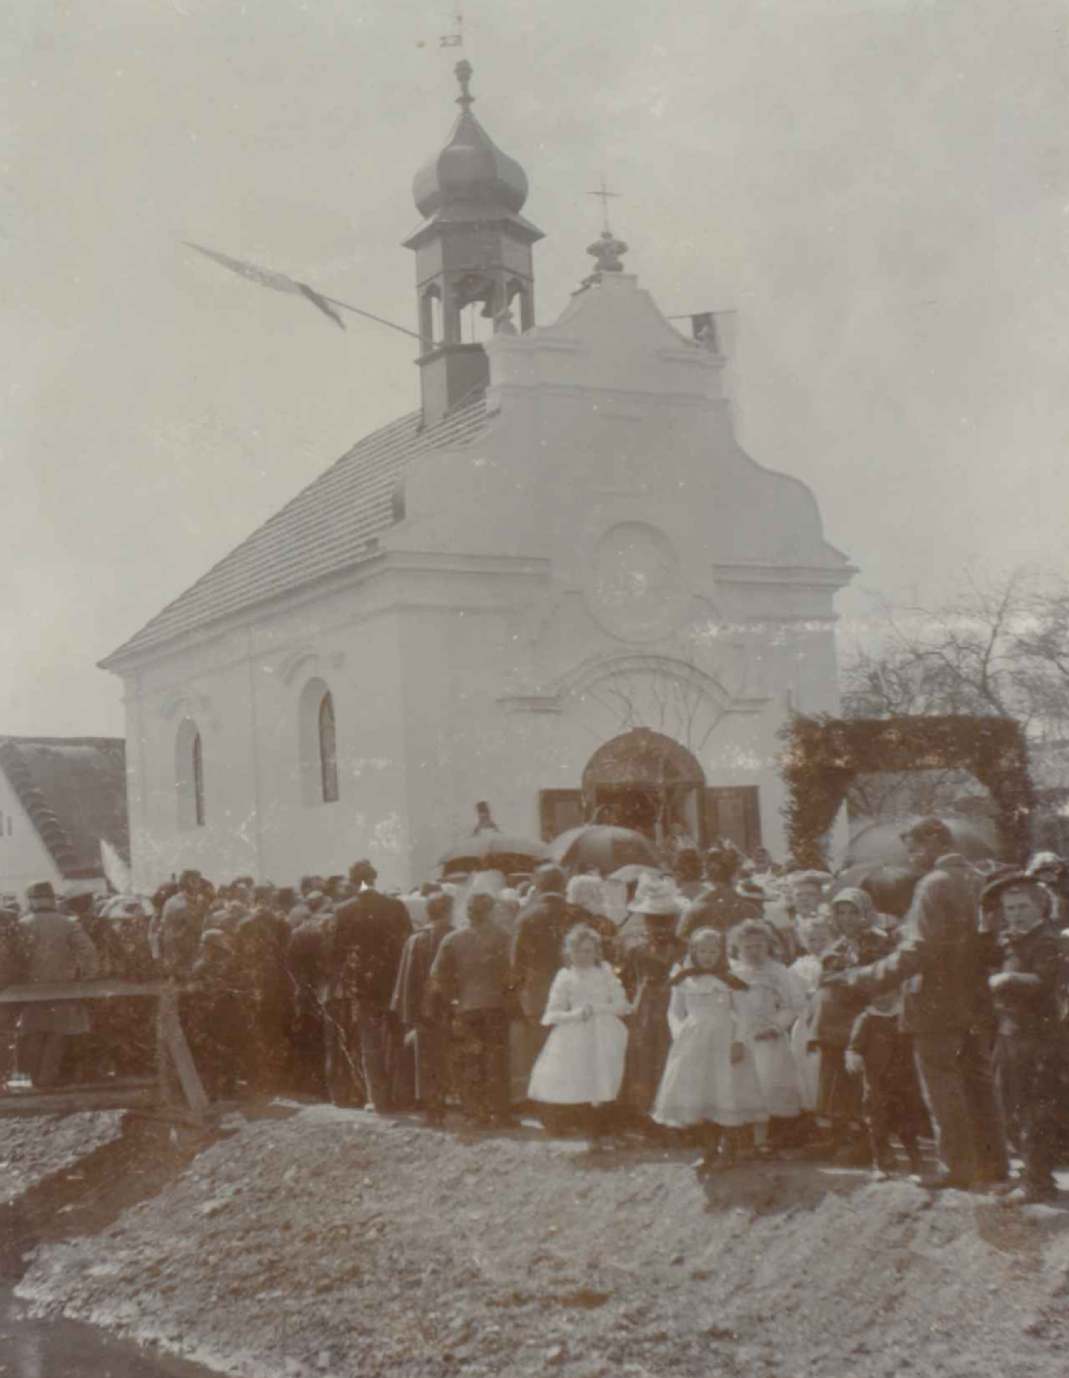
\includegraphics[width=\textwidth, height=\textheight, keepaspectratio]{080-a-vysveceni_kaple}
\caption{Vysvěceni kaple sv. Vojtěcha ve Výrově 27. 4. 1902, postavené na podnět rodiny Prusíků}
\label{fig:080-a-vysveceni_kaple}
\end{figure}

\begin{figure}
\centering
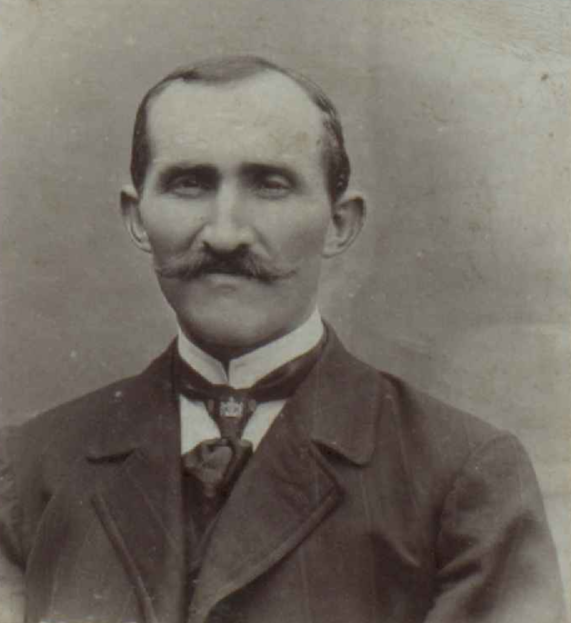
\includegraphics[width=\textwidth, height=\textheight, keepaspectratio]{080-b-vaclav_stefl}
\caption{Václav Štefl, vnuk Marie Prusíkové provdané Šteflové ve Výrově. Po Vojtěchu Prusíkovi byl od roku 1912 starostou obce (1878 – 1918)}
\label{fig:080-b-vaclav_stefl}
\end{figure}

\end{document}
